%
% float.tex
%
% (c) 2020 Prof Dr Andreas Müller, Hochschule Rapperswil
%
\begin{frame}[fragile]
\frametitle{Floating Point Format}

\definecolor{darkgreen}{rgb}{0,0.6,0}

Darstellung einer beliebigen rellen Zahl in der Form
\[
{\color{blue}\pm}
{\color{red}
m.mmmmmmm}
\cdot
2^{\color{darkgreen}xxxxxx}
\]
\ifthenelse{\boolean{presentation}}{
\vspace{-20pt}
}{}

\uncover<2->{
\begin{center}
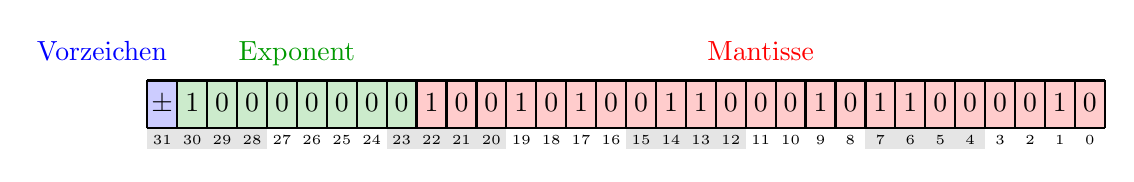
\begin{tikzpicture}[>=latex,thick,scale=0.38]

\definecolor{darkgreen}{rgb}{0,0.6,0}
\fill[color=blue!20]      (0,-0.8) rectangle (1,0.8);
\fill[color=darkgreen!20] (1,-0.8) rectangle (9,0.8);
\fill[color=red!20]       (9,-0.8) rectangle (32,0.8);

\node[color=blue]      at ( 1  ,0.8) [above left] {Vorzeichen\strut};
\node[color=darkgreen] at ( 5  ,0.8) [above] {Exponent\strut};
\node[color=red]       at (20.5,0.8) [above] {Mantisse\strut};

\fill[color=gray!20] ( 0,-0.8) rectangle ( 4,-1.5);
\fill[color=gray!20] ( 8,-0.8) rectangle (12,-1.5);
\fill[color=gray!20] (16,-0.8) rectangle (20,-1.5);
\fill[color=gray!20] (24,-0.8) rectangle (28,-1.5);

\foreach \k in {0,...,31}{
        \node at ({31.5-\k},{-1.2}) {\tiny \k};
}

\draw (0,0.8)--(32,0.8);
\foreach \x in {0,...,32}{
        \draw (\x,-0.8)--(\x,+0.8);
}
\draw (0,-0.8)--(32,-0.8);

\def\feld#1#2{
\node at ({#1+0.5},0) {$\mathstrut #2$};
}

\feld{0}{\pm}

\feld{1}{1}
\feld{2}{0}
\feld{3}{0}
\feld{4}{0}
\feld{5}{0}
\feld{6}{0}
\feld{7}{0}
\feld{8}{0}

\feld{9}{1}
\feld{10}{0}
\feld{11}{0}
\feld{12}{1}
\feld{13}{0}
\feld{14}{1}
\feld{15}{0}
\feld{16}{0}
\feld{17}{1}
\feld{18}{1}
\feld{19}{0}
\feld{20}{0}
\feld{21}{0}
\feld{22}{1}
\feld{23}{0}
\feld{24}{1}
\feld{25}{1}
\feld{26}{0}
\feld{27}{0}
\feld{28}{0}
\feld{29}{0}
\feld{30}{1}
\feld{31}{0}

\end{tikzpicture}
\end{center}}

\ifthenelse{\boolean{presentation}}{
\vspace{-15pt}
}{}

\uncover<3->{

\begin{center}
\renewcommand\arraystretch{1.15}
\begin{tabular}{|l|>{$}l<{$}|>{$}l<{$}|>{$}l<{$}|}
\hline
&\texttt{float}&\texttt{double}&\texttt{long double}\\
\hline
kleinste darstellbare Zahl    &
        1.17549\cdot 10^{-38}&2.22507\cdot 10^{-308}&3.3621\cdot 10^{-4932}\\
grösste darstellbare Zahl     &
        3.40282\cdot10^{38} &1.79769\cdot10^{308} &1.18973\cdot10^{4932}\\
$\varepsilon$                 &
        1.19209\cdot 10^{-7}&2.22045\cdot 10^{-16}&1.0842\cdot 10^{-19}\\
kleinster Exponent            & -125&-1021&-16381\\
grösster Exponent             & 128&1024&16384\\
kleinste denormalisiert Zahl: &
        1.4013\cdot 10^{-45}&4.94066\cdot 10^{-324}&3.6452\cdot 10^{-4951}\\
\hline
\end{tabular}
\end{center}

}

\end{frame}

